\newcommand{\Instance}{\mathcal{I}}
\newcommand{\Beg}{\textit{beg}}
\newcommand{\End}{\textit{end}}
\newcommand{\Left}{\textit{left}}
\newcommand{\Right}{\textit{right}}
\newcommand{\Down}{\textit{down}}
\newcommand{\Up}{\textit{up}}
\newcommand{\Init}{\textit{init}}
\newcommand{\Final}{\textit{final}}


\section{\EXPSPACE-hardness of MC for $\BE$}\label{sec:BEhard}

In the previous section we have seen that MC for $\HS$ can be decided in nonelementary time. 
Obviously, this does \emph{not} imply that such problem is \emph{provably} nonelementary, meaning that no algorithm with elementary complexity may exist for it. Currently, \emph{the existence of such an algorithm is still an open issue}.

Conversely, the best complexity lower bound known to date is $\EXPSPACE$-hardness. This derives from the $\HS$ fragment $\BE$, whose modalities can express properties of both interval prefixes and suffixes
simultaneously: % , which is known to be critical as far as it concerns computational complexity.
we now prove that the MC problem for $\BE$
is $\EXPSPACE$-hard; since MC for full $\HS$ is clearly at least as hard as MC for $\BE$, such a lower bound immediately propagates to full $\HS$. 
The result is obtained by a polynomial-time reduction from a \emph{domino-tiling problem for grids with rows of single exponential length}~\cite{harel92} to MC for $\BE$. 

We start with the definition of the domino-tiling problem.
%
An instance $\Instance$ of a domino-tiling problem for grids with rows of single exponential length is a tuple $\Instance =\tupleof{C,\Delta,n,d_\Init,d_\Final}$, where $C$ is a finite set of colors, $\Delta \subseteq C^{4}$ is a set of tuples $\tupleof{c_\Down,c_\Left,c_\Up,c_\Right}$ of four colors, called \emph{domino-types}, $n>0$ is a  natural number encoded in \emph{unary},
and $d_\Init,d_\Final\in\Delta$ are two distinguished domino-types (respectively, the initial and final domino-types).
The \emph{size} of $\Instance$ is defined as $|C|+|\Delta|+n$.

\begin{figure}[b]
    \centering
    \resizebox{\linewidth}{!}{\begin{tikzpicture}[node distance=0 cm,outer sep = 0pt]

%\draw[use as bounding box] (-1,301) rectangle (16,200);

\tikzstyle{cella}=[draw, rectangle,  minimum height=0.7cm, minimum width={width("dddddd")},anchor=south west];
\tikzstyle{dcella}=[draw, rectangle, dashed, minimum height=0.7cm, minimum width={width("dddddd")},anchor=south west];
%
\node[cella] (k-0) at (0,300) {$d^k_0$};
\node[cella] (k-1) [right = of k-0] {$d^k_1$};
\node[cella] (k-2) [right = of k-1] {$d^k_2$};
\node[dcella] (k-3) [right = of k-2] {};
\node[dcella] (k-4) [right = of k-3] {};
\node[dcella] (k-5) [right = of k-4] {};
\node[cella] (k-6) [right = of k-5] {$d^k_{2^n-2}$};
\node[cella] (k-7) [right = of k-6] {$d^k_{2^n-1}$};
%
\node[dcella] (k1-4) [below = of k-4] {};
\node[cella] (k2-4) [below = of k1-4] {$d^{j+1}_i$};
\node[cella] (k3-4) [below = of k2-4] {$d^{j}_i$};
\node[cella] (k4-4) [below = of k3-4] {$d^{j-1}_i$};
\node[cella] (k3-3) [left = of k3-4] {$d^{j}_{i-1}$};
\node[cella] (k3-5) [right = of k3-4] {$d^{j}_{i+1}$};
\node[dcella] (k5-4) [below = of k4-4] {};
%
%\node[cella] (k-0)  {$d^k_0$};
\node[dcella] (1-4) [below = of k5-4] {};
\node[dcella] (1-5) [right = of 1-4] {};
\node[dcella] (1-3) [left = of 1-4] {};
\node[cella] (1-2) [left = of 1-3] {$d^0_2$};
\node[cella] (1-1) [left = of 1-2] {$d^0_1$};
\node[cella] (1-0) [left = of 1-1] {$d^0_0$};
\node[cella] (1-6) [right = of 1-5] {$d^0_{2^n-2}$};
\node[cella] (1-7) [right = of 1-6] {$d^0_{2^n-1}$};
%
 \node [align=left,red](13) [left = of 1-0] {$d_{init}$};
 \node [align=left,red](13) [right = of k-7] {$d_{final}$};
%
\node[cella] (k-k) at (10.9,298) {$d^j_i$};
\node [align=left,red] [left = of k-k] {$[d^j_i]_\Left$};
\node [align=left,red] [right = of k-k] {$[d^j_i]_\Right$};
\node [align=left,red] [below = of k-k] {$[d^j_i]_\Down =$};
\node [align=left,red] [above = of k-k] {$[d^j_i]_\Up$};
%
\node[cella] (k-k-1) at (10.9,296) {$d^{j-1}_i$};
\node [align=left,red] [above = of k-k-1] {$[d^{j-1}_i]_\Up$};
%
\node[dcella] (i-0) [below = of k-0] {};
\node[dcella] (i-1) [below = of i-0] {};
\node[dcella] (i-2) [below = of i-1] {};
\node[dcella] (i-3) [below = of i-2] {};
\node[dcella] (i-4) [below = of i-3] {};
%
\node[dcella] (j-0) [below = of k-7] {};
\node[dcella] (j-1) [below = of j-0] {};
\node[dcella] (j-2) [below = of j-1] {};
\node[dcella] (j-3) [below = of j-2] {};
\node[dcella] (j-4) [below = of j-3] {};

\end{tikzpicture}
}
%    \vspace{-0.4cm}
    \caption{A (generic) instance of the domino-tiling problem, where $d^i_j$ denotes $f(i,j)$.}\label{fig:til}
\end{figure}

Intuitively, a tiling of a grid is a color labelling of the edges of each cell (see Figure~\ref{fig:til}).
%
Formally, a \emph{tiling of $\Instance$}  is a mapping $f:[0,k]\times [0,2^{n}-1] \rightarrow \Delta$, for some $k\geq 0$, that satisfies the following constraints:
%
\begin{itemize}
  \item two adjacent cells in a row have the same color on the shared edge, namely, for all $(i,j)\in [0,k]\times [0,2^{n}-2]$,
   $[f(i,j)]_{\Right}=[f(i,j+1)]_{\Left}$ (\emph{horizontal requirement});
  \item two adjacent cells in a column have the same color on the shared edge, namely, for all $(i,j)\in [0,k-1]\times [0,2^{n}-1]$,
   $[f(i,j)]_{\Up}=[f(i+1,j)]_{\Down}$ (\emph{vertical requirement});
  \item $f(0,0)=d_\Init$ (\emph{initialization requirement}) and $f(k,2^{n}-1)=d_\Final$ (\emph{acceptance requirement}).
\end{itemize}
%

Checking the existence (respectively, non-existence) of a tiling of $\Instance$ is an $\EXPSPACE$-complete problem~\cite{harel92}.

%Since, clearly, MC for full $\HS$ is at least as hard as MC for $\BE$, the stated lower-bound immediately propagates to MC for formulas of full $\HS$.
%\begin{proof}
%
%Theorem~\ref{theorem:lowerBoundBE} is proved by a polynomial-time reduction from a domino-tiling problem for grids with rows of single exponential length~\cite{harel92}.

We now show how the domino-tiling problem can be reduced in polynomial time to the MC problem for $\BE$.
In particular, we show how to build in polynomial time a finite Kripke structure $\Ku_\Instance$ and a $\BE$ formula $\varphi_\Instance$ such that there exists an initial trace of $\Ku_\Instance$ satisfying $\varphi_\Instance$ if and only if there exists a tiling of $\Instance$. Hence, $\Ku_\Instance\models\neg\varphi_\Instance$ if and only if there is no tiling of $\Instance$.
%and  Theorem~\ref{theorem:lowerBoundBE} follows.

The encoding of tilings exploits the set of proposition letters $\Prop = \Delta \cup \{\$,0,1\}$.
%to encode tilings of $\Instance$:
%\[
%\Prop = \Delta \cup \{\$,0,1\}
%\]
%
Proposition letters in $\{0,1\}$  are used for the binary encoding of the value of an $n$-bit counter numbering the cells of a row of a  tiling, while the proposition letter $\$$ is used as a separator.
In particular, a cell with content $d\in\Delta$ and column number $j\in [0,2^{n}-1]$ is encoded by the word of length $n+1$ over $\Prop$
given by $d \,b_1\cdots b_n$,
 where $b_1 \cdots b_n$ is the binary encoding of the column number $j$ ($b_n$ being the most significant bit). A row is then represented by the word listing the encodings of cells from left to right, and a tiling $f$  consisting of  $k+1$ rows is encoded by the finite word $r_0 \$ r_1 \cdots \$ r_k$, where $r_i$ is the encoding of the
  $i$-th row of $f$, for all $i\in [0,k]$. See Figure~\ref{fig:row} for a graphical account of a word encoding of a tiling.
  
\begin{figure}[tb]
    \centering
    \resizebox{\linewidth}{!}{\newcommand{\cellTwo}[2]{
    \begin{tabular}{c|c}
        \rule[-1ex]{0pt}{3.5ex}
    #1 & #2 \\
    \end{tabular}}

\newcommand{\cellOne}[1]{
    \begin{tabular}{c}
		\rule[-1ex]{0pt}{3.5ex}
		#1
	\end{tabular}}
	
	

\begin{tikzpicture}[node distance=0 cm,->,>=stealth',shorten >=1pt,auto,semithick,main node/.style={rectangle,draw, inner sep=0pt}]  

\tikzstyle{gray node}=[fill=gray!30]
%
 \node [main node](0) at (-4,0) {\cellTwo{$d^0_0$}{$0\cdots 00$}};
 \node [main node](1) [right = of 0] {\cellTwo{$d^0_1$}{$1\cdots 00$}};
\node [main node](11) [right = of 1] {\cellOne{$\cdots$}};
 \node [main node](2) [right = of 11] {\cellTwo{$d^0_{2^n-1}$}{$1\cdots 11$}};
 \node [main node, red](3) [right = of 2]  {\cellOne{\$}};
 %
  \node [main node](4) [right = of 3]  {\cellTwo{$d^1_0$}{$0\cdots 00$}};
   \node [main node](5) [right = of 4]  {\cellTwo{$d^1_1$}{$1\cdots 00$}};
\node [main node](55) [right = of 5] {\cellOne{$\cdots$}};
   \node [main node](6) [right = of 55]  {\cellTwo{$d^1_{2^n-1}$}{$1\cdots 11$}};
   \node [main node, red](7) [right = of 6]  {\cellOne{\$}};
   \node (8) [right = of 7] {\Large $\cdots$};
   
   %
   \node [align=left,red](10) [below = of 0] {column $0$};
   \node [align=left,red](11) [below = of 1] {column $1$};
   \node [align=left,red](12) [below = of 2] {column $2^n - 1$};
   %
   \node [align=left,red](13) [below = of 4] {column $0$};
   \node [align=left,red](14) [below = of 5] {column $1$};
   \node [align=left,red](15) [below = of 6] {column $2^n - 1$};
   %
 \node [align=left,red](20) at (-4,1.2) {row $0$};
  \node [align=left,red](20) at (5.2,1.2) {row $1$};
 
\draw [{|-|},dashed,red,thick] (-5.2,1) -- (3.5,1);
\draw [{|-|},dashed,red,thick] (4.1,1) -- (12.8,1);   


%\path
%(10) edge [swap] node {} (0)
%(11) edge [swap] node {} (1)
%(12) edge [swap] node {} (2)
%(13) edge [swap] node {} (4)
%(14) edge [swap] node {} (5)
%(15) edge [swap] node {} (6);
%    \path
%    (1) edge [swap] node {hardness} (0) 
%    (0) edge  [out=150,in=190] node {hardness} (5.south)
%    (4.west) edge [swap,near end] node {hardness} (3.east)
%    (4.west) edge [near end] node {hardness} (53.east)
%    (2.north east) edge [swap,out=370,in=170] node {upper-bound} (22.north west)
%    (22.south west) edge [swap,out=190,in=-10] node {hardness} (2.south east)
%    (9) edge [swap] node {hardness} (10)
%    (21.north) edge node {hardness} (31.south)
%    (1.west) edge [swap] node {hardness} (32.south);
%    
%    \draw [dashed,-,red,thick] (-6.5,4) -- (6,4);
%    \draw [dashed,-,gray] (-6.5,-2.5) -- (6,-2.5);
%    \draw [dashed,-,gray] (-6.5,-0.5) -- (6,-0.5);
%    
%    \node[align=left](50) at (4,-5) {
%    $^1$ \cite{MMMPP15}, 
%    $^2$ \cite{MMP15}, 
%    $^3$ \cite{MMP15B}, 
%    $^4$ \cite{MMPS16}};

\end{tikzpicture}}
    \vspace{-0.4cm}
    \caption{Encoding of a tiling as a word, where $d^i_j$ denotes $f(i,j)$.}\label{fig:row}
\end{figure}

%\paragraph{Construction of $\Ku_\Instance$ and $\varphi_\Instance$}
The Kripke structure $\Ku_\Instance$ is trivially defined as
 \[
 \Ku_\Instance = \tpl{\Prop, \Prop, \Prop\times \Prop, \Lab,d_\Init}
 ,\]
 where $\Lab(p)=\{p\}$, for each $p\in\Prop$. Thus, the initial traces of $\Ku_\Instance$ correspond to the finite words over $\Prop$ which start with the initial domino type $d_\Init$.
 
In order to build the $\BE$ formula $\varphi_\Instance$, we use some auxiliary formulas, namely, $\Length_i$, $\Beg(p)$, $\End(p)$, $\phi_{\textit{cell}}$, and $\theta_j(b,b')$, where $i\in [1,2n+2]$, $j\in [2,n+1]$, $p\in \Prop$, and $b,b'\in \{0,1\}$.

The formula  $\Length_i$, already presented in Example~\ref{example:length}, has size linear in $i$ and characterizes the traces having length $i$: %It can be expressed as follows:
\[
\Length_i= \hsBu^{i} \bot \wedge \hsB^{i-1} \top.
\]
The formula $\Beg(p)$ (resp., $\End(p)$) captures the traces of $\Ku$ which start (resp., end) in the state $p$:
\[
\Beg(p)= (p\wedge \Length_1) \vee \hsB(p\wedge \Length_1),
\quad
\End(p)= (p\wedge \Length_1) \vee \hsE(p\wedge \Length_1).
\]
The formula $\phi_{\textit{cell}}$ captures the traces of $\Ku_\Instance$ which encode cells:
\[
\phi_{\textit{cell}}= \Length_{n+1}\wedge \Big(\displaystyle{\bigvee_{d\in \Delta} \Beg(d)}\Big)\wedge \hsEu(\Beg(0)\vee \Beg(1)).
\]
%
Finally, for all $j\in [2,n+1]$ and $b,b'\in \{0,1\}$, the formula $\theta_j(b,b')$ is defined as:
\[
\theta_j(b,b')= \hsB(\Length_j \wedge \End(b))\wedge \hsE(\Length_{n-j+2} \wedge \Beg(b')).
\]
It is satisfied by a trace $\rho$ if $|\rho|\geq j+1$, $|\rho|\geq n-j+3$, $\rho(j)= b$, and $\rho(|\rho|-n+j-1)=b'$. In particular, for a trace $\rho$ starting with a cell $c$ and ending with a cell $c'$, $\theta_j(b,b')$ is satisfied by $\rho$ if the $(j-1)$-th bit of $c$ is $b$ and the $(j-1)$-th bit of $c'$ is $b'$. See Figure \ref{fig:thetaj} for an example.
\begin{figure}[t]
    \centering
    \scalebox{0.4}{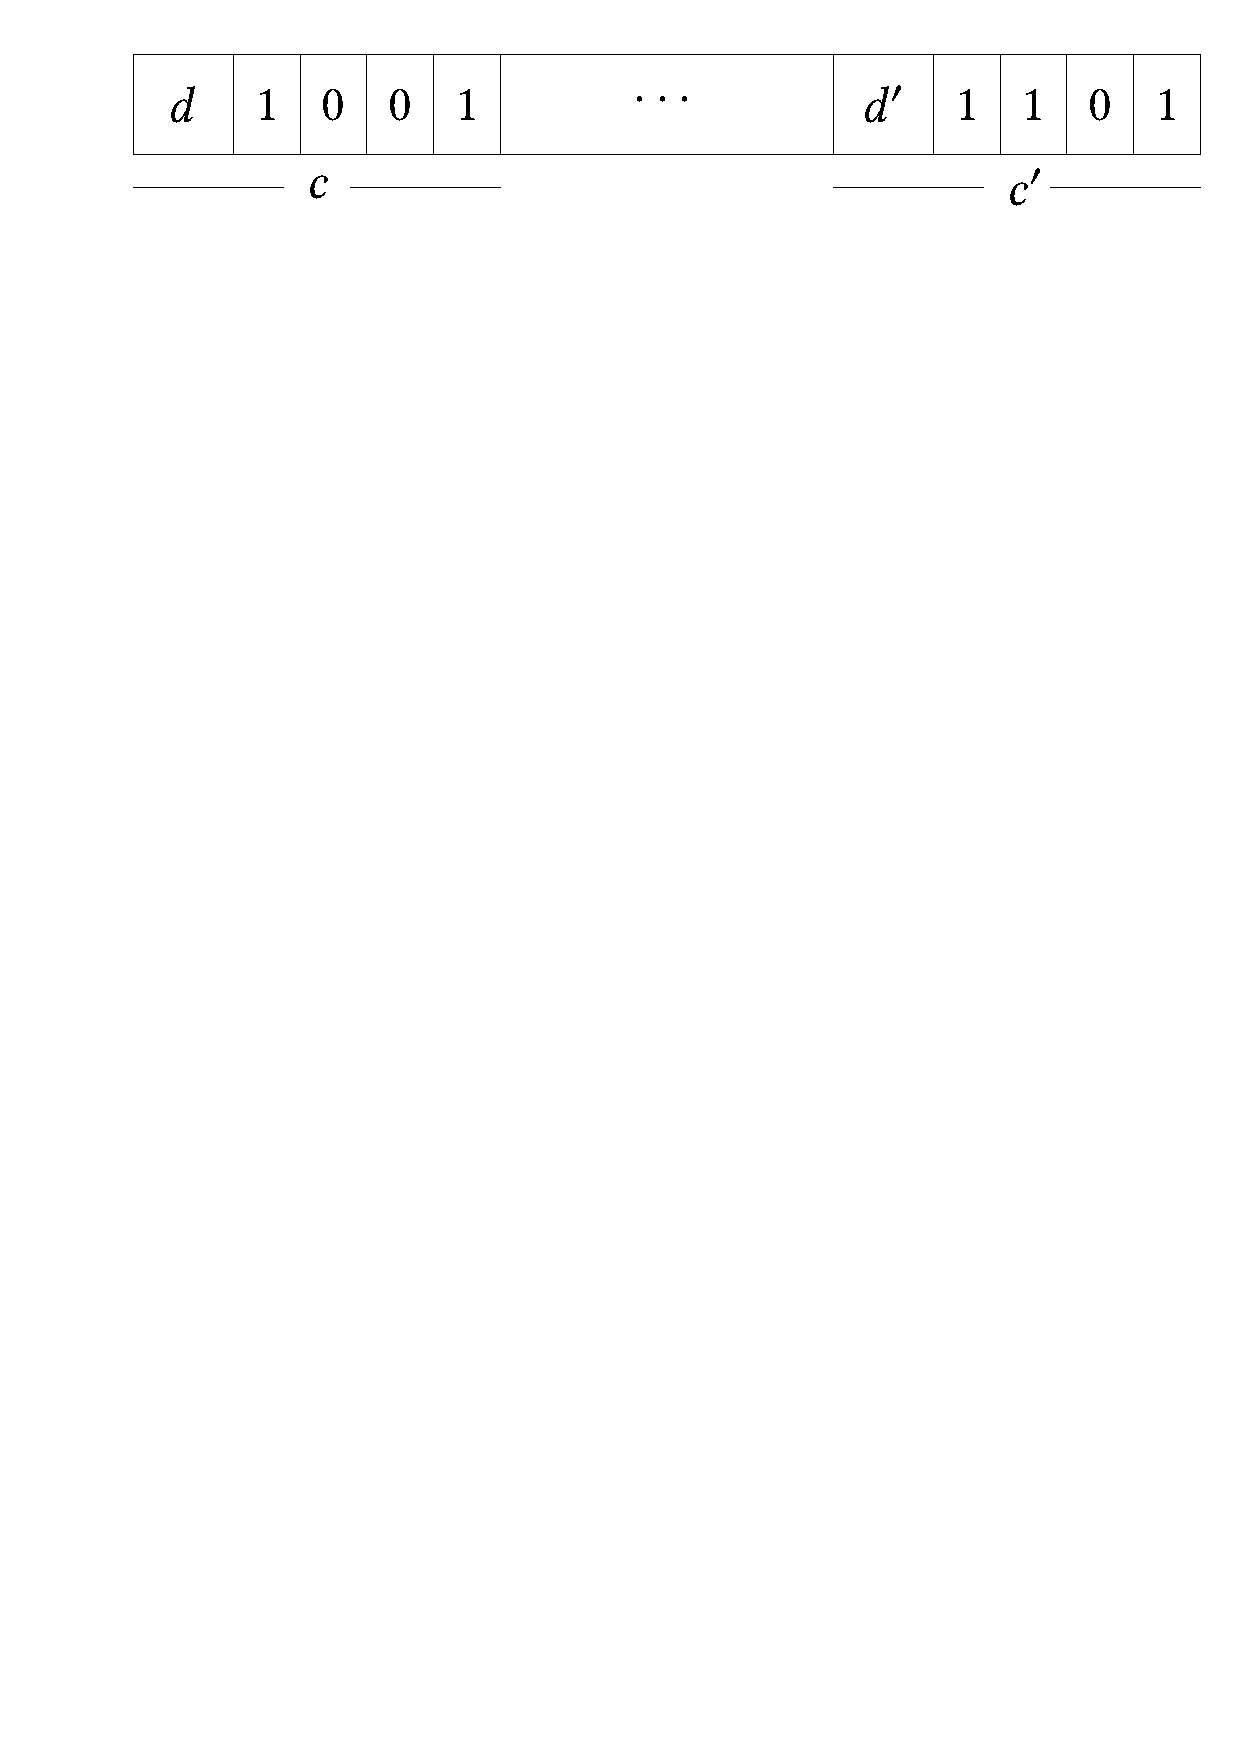
\includegraphics{Chaps/Intro/thetaj.pdf}}
    \caption{Encoding of a trace $\rho$ starting with a cell $c=(d\, 1001)$ and ending with a cell $c'=(d'\, 1101)$ (here, $n=4$). The formula $\theta_2(1,1)$ is satisfied by $\rho$, while $\theta_3(1,0)$ is not.}
    \label{fig:thetaj}
\end{figure}

Additionally, we use the derived operator $\hsG$ and its dual $\hsGu$, which allow us to select  arbitrary subtraces of the given trace, including the trace itself:
\[
\hsG\psi= \psi \vee \hsB\psi \vee \hsE\psi \vee \hsB\hsE\psi.
\]

The formula $\varphi_\Instance$ is defined as follows:
\[
\varphi_\Instance= \varphi_{\textit{b}} \wedge \varphi_{\textit{req}}\wedge \varphi_{\textit{inc}}\wedge \varphi_{\textit{rr}}\wedge \varphi_{\textit{rc}}.
\]
The conjunct $\varphi_{\textit{b}}$ checks that the given trace starts with a cell with content $d_\Init$ and column number $0$, and ends with a cell with content $d_\Final$
and column number $2^{n}-1$:
\[
\varphi_{\textit{b}} = \hsB\phi_{\textit{cell}}\wedge \Beg(d_\Init) \wedge  \hsE(\phi_{\textit{cell}} \wedge \Beg(d_\Final)) \wedge
\displaystyle{\bigwedge_{j=2}^{n+1}}\theta_j(0,1). 
\]
%
The conjunct $\varphi_{\textit{req}}$ ensures the following two requirements:
$(i)$ each occurrence of $\$$ in the given trace is followed by a cell with column number $0$ and
$(ii)$ each cell $c$ in the given trace is followed either by another cell, or by the separator $\$$, and in the latter case $c$ has column number $2^{n}-1$.
%
The first requirement is encoded by the formula: % follows:
\[
\hsGu\bigl((\Length_{n+2} \wedge \Beg(\$)) \longrightarrow \hsE(\phi_{\textit{cell}}\wedge \hsEu\Beg(0))\bigr);
\]
the second one by the formula:
\begin{multline*}
\hsGu\Bigl\{(\Length_{n+2} \wedge \displaystyle{\bigvee_{d\in \Delta}} \Beg(d)) \longrightarrow\\
\Bigl(\hsB\phi_{\textit{cell}} \,\wedge\,  (\End(\$)\vee \displaystyle{\bigvee_{d\in \Delta}} \End(d))\, \wedge\, (\End(\$) \longrightarrow \hsEu(\Beg(\$)\vee \Beg(1)))\Bigr)\Bigr\}.
\end{multline*}
%
The conjunct $\varphi_{\textit{inc}}$  checks that adjacent cells along the given trace have consecutive columns numbers:
%
\[
\varphi_{\textit{inc}} = \hsGu\Bigl( \phi_{\textit{two\_cells}} \longrightarrow \displaystyle{\bigvee_{j=2}^{n+1}}\bigl[\theta_j(0,1)\wedge \bigwedge_{h=2}^{j-1}\theta_h(1,0) \wedge \bigwedge_{h=j+1}^{n+1}\bigvee_{b\in\{0,1\}}\theta_h(b,b)\bigr]\Bigr ),
\]
where $\phi_{\textit{two\_cells}}$ is given by
$
\Length_{2n+2}\wedge  \hsB\phi_{\textit{cell}}\wedge  \hsE\phi_{\textit{cell}}
$.
%
Note that $\varphi_{\textit{req}}$ and $\varphi_{\textit{inc}}$ ensure that column numbers are correctly encoded.

The conjunct $\varphi_{\textit{rr}}$  checks that adjacent cells in a row   have the same color on the shared edge:
\[
\varphi_{\textit{rr}} = \hsGu\Bigl( \phi_{\textit{two\_cells}} \longrightarrow\quad \smashoperator{\bigvee_{(d,d')\in \Delta\times \Delta\mid d_{\Right}= d'_{\Left}}} \quad (\Beg(d) \wedge \hsE(\Length_{n+1}\wedge \Beg(d')))\Bigr ) .
\]
%
Finally, the conjunct   $\varphi_{\textit{rc}}$  checks that adjacent cells in a column  have the same color on the shared edge.
For this, it suffices to require that
the following condition holds:
\begin{itemize}
  \item for each subtrace of the given one containing exactly one occurrence of $\$$, starting with a cell $c$, and ending with a cell $c'$, if $c$ and $c'$ have the same column number, then $d_{\Up}= d'_{\Down}$, where $d$ (respectively, $d'$) is the content of $c$ (respectively, $c'$).
\end{itemize}
%
Accordingly, the formula $\varphi_{\textit{rc}}$ is defined as follows, where we use the formulas $\theta_j(b,b)$, with $j\in [2,n+1]$ and $b\in \{0,1\}$, to express that $c$ and $c'$ have the same column number:
\begin{multline*}
  \varphi_{\textit{rc}} = \hsGu\Bigl\{\,\, \Big(\phi_{\textit{one}}(\$) \,\,\wedge \,\, \hsB\phi_{\textit{cell}} \,\,\wedge \,\, \hsE\phi_{\textit{cell}} \,\,\wedge \,\, \displaystyle{\bigwedge_{j=2}^{n+1}\bigvee_{b\in \{0,1\}}}\theta_j(b,b)\,\,\Bigr)\\
  \longrightarrow \smashoperator[r]{\bigvee_{(d,d')\in \Delta\times \Delta\mid d_{\Up}= d'_{\Down}}}\quad (\Beg(d) \wedge \hsE(\Length_{n+1}\wedge \Beg(d')))\,\,\,\Bigr\},
\end{multline*}
%
where $\phi_{\textit{one}}(\$)$ is defined as
\[
(\hsB\End(\$))\,\,\wedge\,\, \neg(\hsB(\End(\$) \wedge \hsB\End(\$)))
.\]

The formula $\varphi_\Instance$ has length polynomial in the size of $\Instance$. 
%
By construction, a trace $\rho$ of $\Ku_\Instance$ satisfies $\varphi_\Instance$ if and only if $\rho$ encodes a tiling.
Since the initial traces of $\Ku_\Instance$ are the finite words over $\Prop$ starting with $d_\Init$, it follows that there exists a tiling of $\Instance$ if and only if there exists an initial trace
of $\Ku_\Instance$ which satisfies $\varphi_\Instance$. 

The given reduction proves the following theorem. %, concluding the section.
%of Theorem~\ref{theorem:lowerBoundBE} is finished.

\begin{theorem}\label{theorem:lowerBoundBE} The MC problem for $\BE$ formulas over finite Kripke structures is \EXPSPACE-hard (under polynomial-time reductions).
\end{theorem}
%\end{proof}


Before concluding the section,
we would like to comment on the complexity gap deriving from the upper and lower bounds proved for $\HS$ (and $\BE$) MC.

Let us start by introducing \emph{star-free regular expressions} over a finite alphabet $\Sigma$, with $|\Sigma|\geq 2$, that are defined by the grammar
\[r::= \emptyset \mid a \mid r \cdot r \mid r \cup r \mid \neg r ,\]
where $a\in\Sigma$.
Every regular expression defines a language $\Lang(r)$ of finite words over $\Sigma$ by induction on its structural complexity
as follows:
%\begin{itemize}
   $\Lang(\emptyset)=\emptyset$,
   $\Lang(a)=\{a\}$,
   $\Lang(r_1\cdot r_2)=\Lang(r_1)\cdot \Lang(r_2)$,
   $\Lang(r_1\cup r_2)=\Lang(r_1)\cup \Lang(r_2)$ and
   $\Lang(\neg r)=\Sigma^*\setminus\Lang(r)$.\footnote{%
   As a standard notation, the dot $\cdot$ represents the concatenation of words, and $\Sigma^*$ (resp., $\Sigma^+$) the set of all possible \emph{finite} (resp., finite and non-empty) words over $\Sigma$.
   } 
%\end{itemize}
It is well-known that the \emph{language-emptiness problem for star-free regular expressions is (provably) nonelementary}~\cite{Stockmeyer:1973,stockmeyer1974} (more properly, \TOWER-complete in the notation of~\cite{Schmitz:2016}), being negation the \lq\lq difficult case\rq\rq.

Let us now slightly modify the definition of these expressions. We consider:
\[r::= \emptyset \mid a \mid r \cdot \Sigma^+ \mid \Sigma^+\cdot r \mid r \cup r \mid \neg r .\]
Again, negation is present and there is no Kleene star (as $\Sigma^+$ can be \lq\lq rewritten\rq\rq{} as $\neg\emptyset$); \emph{concatenation is now weakened}: in fact, $r \cdot \Sigma^+$ and $\Sigma^+\cdot r$ represent right-/left-extensions of a word in $\Lang(r)$ with any (non-empty) word.
To the best of our knowledge, nothing is known about the precise complexity of this variant of star-free regular expressions.

The reader may now be wondering why we care so much about these regular expressions. The answer is given by the following fact:
\emph{there is a trivial reduction from language emptiness for this variant of expressions to $\BE$ MC, and vice versa}.
Intuitively, $r \cdot \Sigma^+$ (resp., $\Sigma^+\cdot r$) can be \lq\lq simulated\rq\rq{} by $\hsB$ (resp., $\hsE$).%
\footnote{It is also worth noting that the \lq\lq general\rq\rq{} concatenation $r\cdot r$ cannot be simulated by $\BE$: the \emph{chop} operator would be needed, which bisects an interval into two consecutive parts/subintervals: $\psi_1\langle C\rangle \psi_2$ predicates $\psi_1$ over the first subinterval and $\psi_2$ over the second.}
%
As an immediate consequence, an improvement on the known (upper or lower) bounds for any of the two problems would immediately propagate to the other.

Unfortunately, the nonelementary lower bound proved for (standard) star-free regular expressions by Stockmeyer in his PhD thesis \cite{stockmeyer1974} cannot be adapted to the variant, failing to encode the so-called \lq\lq \emph{movable rulers}\rq\rq, 
namely, regular expressions that are \lq\lq satisfied\rq\rq{} only by (all) words of a precise length.
Conversely, it is not clear how the (nonelementary) complexity of the standard automata-based algorithm for deciding the emptiness of regular expressions could possibly be lowered by exploiting the weakened concatenation; analogously, the nonelementary algorithm for full $\HS$ MC represents, at the moment, the best algorithm also for $\BE$ MC. 
